\section{实验步骤}

本章节将介绍实验的具体步骤,包括实现距离计算函数、Tiny Image表征函数、KNN分类器函数、K-means聚类函数、词典构造函数、聚类中心匹配函数、Bag of Words表征函数等。

\subsection{实现距离计算函数}

距离计算函数用于计算两个特征向量之间的距离。本实验使用欧氏距离作为距离计算函数,具体实现如下:

\begin{lstlisting}[style=Python]
def pairwise_distances(X, Y):
    return np.linalg.norm(X[:, np.newaxis, :] - Y[np.newaxis, :, :], axis=2)
\end{lstlisting}

该函数接收两个特征向量矩阵$X\in\mathbb{R}^{N\times D}$和$Y\in\mathbb{R}^{M\times D}$,返回一个距离矩阵$D\in\mathbb{R}^{N\times M}$,其中$D_{ij}$表示$X_i$和$Y_j$之间的距离。

\subsection{实现Tiny Image表征函数}

Tiny Image表征是一种简单的图像表征方法,通过将图像缩放到固定大小,然后将图像像素展平,最后对向量进行归一化处理。Tiny Image表征函数的具体实现如下:

\begin{lstlisting}[style=Python]
def get_tiny_images(image_arrays):
    def resize(img, size, keep_aspect_ratio):
        if not keep_aspect_ratio:
            return cv2.resize(img, (size, size))
        h, w = img.shape
        if h > w:
            img = cv2.resize(img, (size, int(size * h / w)))
            return img[(img.shape[0] - size) // 2:(img.shape[0] + size) // 2, :]
        else:
            img = cv2.resize(img, (int(size * w / h), size))
            return img[:, (img.shape[1] - size) // 2:(img.shape[1] + size) // 2]

    def normalize(img):
        img = img.flatten()
        img = img - np.mean(img)
        img = img / np.linalg.norm(img)
        return img
    
    feats = []
    keep_aspect_ratio = False
    size = 16
    for img in image_arrays:
        resized_img = resize(img, size, keep_aspect_ratio)
        feats.append(normalize(resized_img))
    return np.array(feats)
\end{lstlisting}

该函数接收一个图像数组列表,其中每个元素为一个灰度图像矩阵$x\in\mathbb{R}^{H\times W}$,返回一个Tiny Image表征矩阵$X\in\mathbb{R}^{N\times D}$,其中$N$为图像数量,$D$视图像缩放后的大小而定。resize函数用于缩放图像,可以设置是否保持长宽比;normalize函数用于对图像向量进行中心化和归一化处理。

\subsection{实现KNN分类器函数}

KNN分类器是一种简单的无需训练的分类方法,通过计算新数据点与训练数据点之间的距离,找到最近的K个数据点,然后根据这K个数据点的类别,通过投票的方式决定新数据点的类别。KNN分类器函数的具体实现如下:

\begin{lstlisting}[style=Python]
def nearest_neighbor_classify(train_image_feats, train_labels,
                              test_image_feats, k=3):
    test_labels = []
    dists = pairwise_distances(test_image_feats, train_image_feats)
    topk_inds = np.argsort(dists, axis=1)[:, :k]
    topk_labels = np.array(train_labels)[topk_inds]

    for labels in topk_labels:
        label, count = np.unique(labels, return_counts=True)
        test_labels.append(label[np.argmax(count)])
    
    return test_labels
\end{lstlisting}

该函数接收训练数据特征矩阵$X_{train}\in\mathbb{R}^{N_{train}\times D}$、训练数据标签列表$Y_{train}\in\mathbb{R}^{N_{train}}$、测试数据特征矩阵$X_{test}\in\mathbb{R}^{N_{test}\times D}$和K值$k$,返回测试数据标签列表$Y_{test}\in\mathbb{R}^{N_{test}}$。该函数首先计算测试数据与训练数据之间的距离矩阵,然后找到每个测试数据的最近的K个训练数据,最后通过投票的方式决定测试数据的类别。

\subsection{实现K-means聚类函数}

K-means是一种简单的无监督聚类方法,通过迭代更新簇中心,将数据集划分为K个簇。K-means聚类函数的具体实现如下:

\newpage
\begin{lstlisting}[style=Python]
def kmeans(feature_vectors, k, max_iter = 10):
    N, D = feature_vectors.shape
    labels_prev = np.zeros(N)

    # initialization with KMeans++
    inds = [np.random.choice(N)]
    for _ in range(k - 1):
        dists = np.min(pairwise_distances(feature_vectors, feature_vectors[inds]), axis=1)
        probs = dists / np.sum(dists)
        inds.append(np.random.choice(N, p=probs))

    centroids = feature_vectors[inds]
    for _ in range(max_iter):
        # assign labels
        dists = pairwise_distances(feature_vectors, centroids)
        labels = np.argmin(dists, axis=1)
        # check convergence
        if np.all(labels == labels_prev):
            break
        labels_prev = labels
        # update centroids
        for i in range(k):
            if np.sum(labels == i) == 0:
                continue
            centroids[i] = np.mean(feature_vectors[labels == i], axis=0)
    return centroids
\end{lstlisting}

该函数接收特征向量矩阵$X\in\mathbb{R}^{N\times D}$和簇的数量$K$,返回簇中心矩阵$C\in\mathbb{R}^{K\times D}$。需要注意的是,为了通过单元测试,该函数采用KMeans++初始化方法,具体来说,首先随机选择一个数据点作为第一个簇中心,然后在剩余数据点中根据到当前簇中心的距离确定概念,抽取下一个簇中心。

在完成初始化之后,K-means算法通过迭代更新簇中心和分配数据点的簇标签,首先计算每个数据点到簇中心的距离,然后将数据点分配到最近的簇中心,接着更新簇中心为分配到该簇的数据点的均值。当簇标签不再变化时,算法结束。

\subsection{实现词典构造函数}

Bag of Visual Words中的词典是通过对视觉特征进行K-means聚类算法得到的,词典的大小即为聚类的簇的数量。词典构造函数的具体实现如下:

\begin{lstlisting}[style=Python]
def build_vocabulary(image_arrays, vocab_size, stride = 20):
    pad = 10
    keep_ratio = 1.0
    sifts = []
    for img in image_arrays:
        h, w = img.shape
        xx, yy = np.meshgrid(np.arange(pad, w - pad, stride), np.arange(pad, h - pad, stride))
        xx, yy = xx.flatten(), yy.flatten()
        if 0.0 < keep_ratio < 1.0:
            inds = np.random.choice(len(xx), int(len(xx) * keep_ratio), replace=False)
            xx, yy = xx[inds], yy[inds]
        
        img_tensor = torch.from_numpy(np.array(img, dtype='float32'))
        img_tensor = img_tensor.reshape(1, 1, img.shape[0], img.shape[1])
        siftnet_feats = get_siftnet_features(img_tensor, xx, yy)
        sifts.append(siftnet_feats)
                
    sifts = np.concatenate(sifts)
    vocab = kmeans(sifts, vocab_size)
    return vocab
\end{lstlisting}

该函数接收一个图像数组列表,其中每个元素为一个灰度图像矩阵$x\in\mathbb{R}^{H\times W}$,返回一个词典矩阵$V\in\mathbb{R}^{K\times D}$,其中$K$为词典的大小,$D$为特征向量的维度。该函数首先对图像进行SIFT特征提取,然后将所有特征向量拼接在一起,最后通过K-means聚类算法得到若干簇中心作为词典。

其中,SIFT特征通过对图像进行网络采样,之后对每个采样点提取SIFT特征,最后将所有特征向量拼接在一起。

\subsection{实现聚类中心匹配函数}

聚类中心匹配函数用于将特征向量映射到最近的簇中心,具体实现如下:

\begin{lstlisting}[style=Python]
def kmeans_quantize(raw_data_pts, centroids):
    dists = pairwise_distances(raw_data_pts, centroids)
    indices = np.argmin(dists, axis=1)
    return indices
\end{lstlisting}

该函数接收原始数据点矩阵$X\in\mathbb{R}^{N\times D}=\{x_j\}$和簇中心矩阵$C\in\mathbb{R}^{K\times D}$,返回一个索引列表$I\in\mathbb{R}^{N}=\{i_j\}$,其中$i_j$表示$x_j$的映射索引。

\subsection{实现Bag of Words表征函数}

Bag of Words表征是一种常见的图像表征方法,通过对图像的视觉特征进行聚类,然后统计每个视觉单词的出现频率,最后对频率向量进行归一化处理。Bag of Words表征函数的具体实现如下:

\begin{lstlisting}[style=Python]
def get_bags_of_sifts(image_arrays, vocabulary, step_size = 10):
    feats = []
    pad = 10
    for img in image_arrays:
        h, w = img.shape
        xx, yy = np.meshgrid(np.arange(pad, w - pad, step_size), np.arange(pad, h - pad, step_size))
        xx, yy = xx.flatten(), yy.flatten()
        
        img_tensor = torch.from_numpy(np.array(img, dtype='float32'))
        img_tensor = img_tensor.reshape((1, 1, img.shape[0], img.shape[1]))
        siftnet_feats = get_siftnet_features(img_tensor, xx, yy)

        indices = kmeans_quantize(siftnet_feats, vocabulary)
        hist, _ = np.histogram(indices, bins=np.arange(len(vocabulary) + 1))
        hist = hist / np.linalg.norm(hist)
        feats.append(hist)
    
    return np.array(feats)
\end{lstlisting}

该函数接收一个图像数组列表,其中每个元素为一个灰度图像矩阵$x\in\mathbb{R}^{H\times W}$,一个词典矩阵$V\in\mathbb{R}^{K\times D}$,返回一个Bag of Words表征矩阵$X\in\mathbb{R}^{N\times K}$,其中$N$为图像数量,$K$为词典的大小。该函数首先对图像进行SIFT特征提取,同样通过网络采样得到局部特征。之后,将局部特征映射到词典中最近的视觉词,然后统计每个视觉词的出现频率得到频率向量(直方图),最后对频率向量进行归一化处理,得到最终的特征向量表示。

\subsection{运行测试程序}

在实现上述函数之后,可以运行测试程序,对Tiny Image表征、KNN分类器、K-means聚类、词典构造、Bag of Words表征等功能进行测试。通过如下命令启动Jupyter Notebook:

\begin{lstlisting}[style=Bash]
jupyter notebook
\end{lstlisting}

之后,打开实验目录的\texttt{proj3.ipynb}文件,如图\ref{fig:jupyter}所示,点击运行按钮,即可运行测试程序。

\begin{figure}[H]
    \centering
    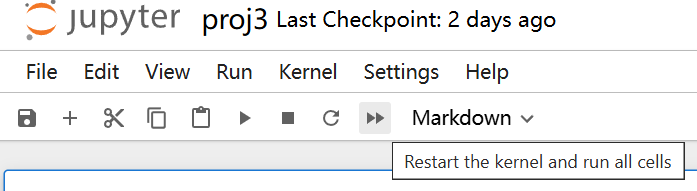
\includegraphics[width=0.5\textwidth]{pics/jupyter.png}
    \caption{Jupyter Notebook运行按钮}
    \label{fig:jupyter}
\end{figure}

如图\ref{fig:unit_test}所示,测试结果显示所有函数均通过测试,实现正确。

% unit1.png / unit2.png / unit3.png / unit4.png / unit5.png
\begin{figure}[H]
    \centering
    \subfigure[Tiny Image表征函数测试结果]{
        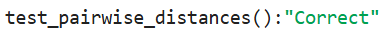
\includegraphics[width=0.3\textwidth]{pics/unit1.png}
    }
    \subfigure[KNN分类器函数测试结果]{
        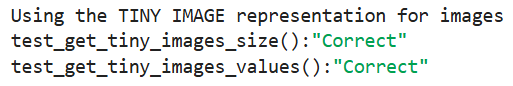
\includegraphics[width=0.3\textwidth]{pics/unit2.png}
    }
    \subfigure[K-means聚类函数测试结果]{
        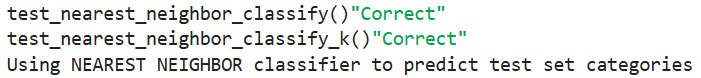
\includegraphics[width=0.3\textwidth]{pics/unit3.png}
    }
    \subfigure[词典构造函数测试结果]{
        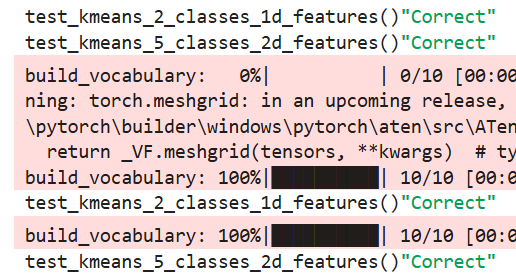
\includegraphics[width=0.3\textwidth]{pics/unit4.png}
    }
    \subfigure[Bag of Words表征函数测试结果]{
        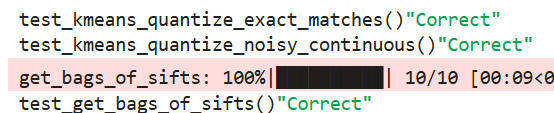
\includegraphics[width=0.3\textwidth]{pics/unit5.png}
    }
    \caption{实验函数单元测试结果}
    \label{fig:unit_test}
\end{figure}